\documentclass[a4paper, 12pt, twoside]{article}
\usepackage[a4paper, top=2.5cm, bottom=2.5cm, left=2.5cm, right=2.5 cm, bindingoffset=0.5cm]{geometry}
\usepackage[onehalfspacing]{setspace}
\usepackage[utf8]{inputenc}
\usepackage[polish]{babel}
\usepackage[T1]{fontenc}
\usepackage{graphicx}
\usepackage{ragged2e}
\usepackage{indentfirst}
\usepackage{csquotes}
\usepackage[backend=biber, maxbibnames=30]{biblatex}
\usepackage{amsmath}
\usepackage{todonotes}
\usepackage{float} % to use figure positioning [H]
\usepackage{multirow} % tabele wielowierszowe komórki
\usepackage{array} % jw
\usepackage{tabularx}
\addbibresource{inz.bib}
\graphicspath{ {./images/} }

\title{System IIoT do zbierania danych pomiarowych}
\date{}

\begin{document}

\clearpage\maketitle %no page number on title page
\thispagestyle{empty}

\listoftodos

\newpage

\tableofcontents

\section{Wstęp}\label{intro}

Systemy informatyczne znajdują obecnie szerokie zastosowanie w wielu przedsiębiorstwach.
Do zadań takich systemów należą przede wszystkim: automatyzacja procesów,
ułatwienie zarządzania zasobami (ludzkimi, materialnymi, finansowymi, dokumentacją, wiedzą),
gromadzenie informacji na temat prowadzonej
działalności na potrzeby raportowania, nadzoru, optymalizacji i rozwoju strategii, a także
usprawnienie komunikacji z klientami i kontrahentami. Korzyści wynikające z wdrożenia
rozwiązań informatycznych wykorzystuje się również w środowisku
przemysłowym. Obok wymienionych zadań (obejmujących szerszy zakres działalności
przedsiębiorstwa) podstawową rolą przemysłowych systemów informatycznych
jest wspomaganie prowadzenia procesów przemysłowych (produkcji przemysłowej).
Istotnym aspektem działania takich systemów
jest zbieranie danych pomiarowych. Dane gromadzone przez zainstalowaną w systemie produkcji
aparaturę pomiarową, jak i wprowadzane przez ludzi lub inne systemy, determinują działanie układów automatyki,
umożliwiają nadzór, diagnostykę, regulację, monitorowanie i wizualizację procesów przemysłowych.
Ponadto stosunkowo duża liczba gromadzonych danych poddana zaawansowanemu przetwarzaniu
(ang. \emph{big data})
może dostarczyć cennej wiedzy w kontekście prowadzenia biznesu.
Wymaganiem charakterystycznym stawianym wobec systemów informatyki przemysłowej
jest konieczność działania w~ramach ograniczeń nakładanych przez specyficzne środowisko.
Należą do nich: determinizm działań i determinizm czasowy, niezawodne funkcjonowanie (odporne
na często niesprzyjające warunki), bezpieczeństwo danych i~urządzeń~\cite{isp}.

Zbieranie znacznej ilości danych w celu ich dalszego przetwarzania wymienia się
wśród głównych zadań Internetu Rzeczy (ang. \emph{Internet of Things}, w skrócie:~IoT).
Jest to koncepcja, w myśl której przedmioty wyposażone w czujniki i/lub elementy
wykonawcze są podłączane do Internetu. Systemy wykorzystujące Internet Rzeczy stały się szczególnie popularne
w ostatnich latach dzięki czynnikom ułatwiającym ich realizację:
znaczący rozwój systemów komputerowych małej i~średniej skali oraz urządzeń mobilnych, upowszechniony
dostęp do Internetu, stopniowe wdrażanie protokołu IPv6, duże postępy w dziedzinie
eksploracji danych, uczenia maszynowego i inteligencji obliczeniowej,
a~także dynamiczny rozwój usług opartych na chmurze obliczeniowej~\cite{intro-to-iot}.
Dziedzina zastosowań IoT jest szeroka, gdyż obejmuje ona urządzenia
o wielu różnych przeznaczeniach. Powszechne stało się używanie określenia ,,inteligenty''
(ang. \emph{smart}) wobec tego typu przedmiotów lub środowisk, w których są one używane.  W~ten sposób
powstały koncepcje inteligentnych gadżetów i urządzeń gospodarstwa domowego,
rolnictwa, logistyki, systemów opieki zdrowotnej, budynków, a nawet miast.
Do obszarów wykorzystania IoT zalicza się także przemysł. Koncepcja ta nosi
nazwę Przemysłowego Internetu Rzeczy (ang. \emph{Industrial Internet of Things}, w skrócie IIoT).
Głównym przeznaczeniem IIoT jest gromadzenie wiedzy na temat procesu przemysłowego,
a~w~konsekwencji --- zwiększanie jego efektywności \cite{iiot-challenges-opportunities-directions}.

Celem niniejszej pracy jest zaprojektowanie systemu informatycznego
wraz z prototypem, którego podstawowym zadaniem jest zbieranie i składowanie danych pomiarowych.
Obszarem zastosowań systemu jest środowisko przemysłowe.
W realizacji projektu kładzie się nacisk na wykorzystanie technologii IoT
oraz chmury obliczeniowej. Źródłem danych w systemie
jest aparatura pomiarowa (czujniki) funkcjonująca w~ramach systemów automatyki i IoT,
inne systemy informatyczne wdrożone w przedsiębiorstwie,
a także pracownicy obsługujący proces przemysłowy (mogą oni monitorować jego działanie
i~wprowadzać wyniki obserwacji do systemu, jak również wyzwalać określone zdarzenia).
Przedmiotem pracy jest ogólne opracowanie architektury
systemu adresujące przedstawiony problem aplikacyjny. Stąd opisane w kolejnych rozdziałach
rozwiązanie teoretyczne abstrahuje od szczegółowych przpyadków użycia, konkretnych urządzeń
technicznych czy technologii. Oczekiwaną cechą systemu jest możliwość dostosowania
do różnych konfiguracji sprzętu i oprogramowania stosowanych w~IoT i~dedykowanych
rozwiązaniach przemysłowych. Jedną z~możliwych implementacji i~jednocześnie weryfikacją
zaproponowanej koncepcji systemu jest wykonany prototyp. Na jego potrzeby zdefiniowano
kilka ściślej sprecyzowanych scenariuszy zastosowania, dokonano wyboru urządzeń
i określonych usług chmurowych, jak również bibliotek i narzędzi programistycznych.

W rozdziale \ref{analiza} przedstawiono przegląd dostępnej literatury związanej z podjętą problematyką.
W pierwszej kolejności omówiono z osobna poszczególne zagadnienia, które
obejmuje temat pracy, przybliżając w ten sposób jego dziedzinę.
Następnie zebrane informacje zestawiono w kontekście realizowanego zadania projektowego,
wskazano możliwe problemy i potencjalne rozwiązania wraz z zarysem architektury
systemu. Opisano również kilka dostępnych na rynku rozwiązań komercyjnych,
które adresują podobny zakres funkcjonalny. W rozdziale \ref{wymagania} sprecyzowano
wymagania funkcjonalne i niefunkcjonalne, które ma realizować projektowany system
oraz zdefiniowano ogólne przypadki użycia.
Opisano również metodykę pracy oraz wybrane narzędzia, technologie i biblioteki użyte do realizacji
prototypu. Rozdział \ref{spec-zew} zawiera informacje dotyczące
wdrażania i~używania systemu, a także wymagań sprzętowych i programowych.
Poruszono również kwestie bezpieczeństwa. W oparciu o zrealizowany prototyp przedstawiono
przykładowe scenariusze korzystania z systemu. W rozdziale \ref{spec-wew} zamieszczono
szczegółowy opis architektury zaprojektowanego systemu. Wymieniono jej poszczególne
komponenty i~omówiono sposoby ich wzajemnej interakcji. Zdefiniowano interfejs
komunikacyjny systemu, przedstawiono sposoby integracji wykorzystanych gotowych
narzędzi z elementami autorskimi. Opisano także rozwiązania
mające na celu poprawę bezpieczeństwa. Rozdział \ref{testy} zawiera
opis stosowanej metodyki testowania i przypadków testowych oraz przedstawia wyniki przeprowadzonych
testów z uwzględnieniem napotkanych problemów. W rozdziale \ref{wnioski} zamieszczono
podsumowanie i wnioski, które nasunęły się po zakończeniu prac nad projektem.
Uzyskany rezultat zestawiono z postawionymi celami i określonymi wymaganiami.
Rozważono również kierunki dalszego rozwoju systemu.


\section{Analiza tematu}\label{analiza}

W niniejszym rozdziale przedstawiono rozważania teoretyczne dotyczące projektowanego
systemu opierające się na analizie dostępnej literatury. Realizowany temat
składa się z czterech zasadniczych zagadnień: systemy do zbierania danych pomiarowych,
systemy informatyczne w przemyśle, IoT i IIoT.  Do każdego z nich odnoszą się
odpowiednio kolejne podrozdziały przedstawiające podstawowe pojęcia, problemy i~rozwiązania
w danej dziedzinie.
W ostatnim podrozdziale dokonano konsolidacji zebranych wiadomości w kontekście
celu pracy, jakim jest opracowanie systemu do zbierania danych pomiarowych
dla środowiska przemysłowego z wykorzystaniem IoT.

\subsection{Systemy informatyczne do zbierania danych pomiarowych} \label{system-do-zbierania-danych}

Zgodnie z encyklopedią \textbf{system informatyczny} to zespół systemów komputerowych,
sieci oraz oprogramowania, których celem zastosowania jest
przetwarzanie informacji \cite{system-informatyczny}.
\textbf{Przetwarzaniem informacji} nazywa się proces akwizycji, utrwalania, udostępniania,
organizacji, interpretacji i wizualizacji informacji \cite{information-science},
\cite{information-processing}. Warto w~tym miejscu doprecyzować pojęcia
\textbf{informacji} oraz \textbf{danych}. Dane są pewną skodyfikowaną reprezentacją
faktów. Natomiast dane, które podlegają intepretacji i nabierają znaczenia
stają się informacją \cite{dane-informacja-wiedza}.

Jednym z możliwych źródeł informacji w systemie informatycznym mogą być
\textbf{systemy do zbierania danych pomiarowych} (system akwizycji danych, ang. \emph{Data Acquisition Systems}, w skrócie: DAQ).
Są to systemy, których rolą jest gromadzenie w formie cyfrowej danych opisujących
zjawiska fizyczne. Systemy DAQ tworzą między innymi następujące komponenty
o odpowiednich przeznaczeniach:
\begin{itemize}
      \itemsep0em
      \item czujniki (sensory, ang. \emph{sensors}) --- przetwarzanie zjawisk fizycznych na analogowy sygnał elektryczny,
      \item przetworniki analogowo-cyfrowe --- konwersja sygnału analogowego na cyfrowy,
      \item sprzęt komputerowy i oprogramowanie --- przetwarzanie informacji.
\end{itemize}
Systemy DAQ stanowią jedno z głównych narzędzi stosowanych przez naukowców i~inżynierów
na potrzeby testów, pomiarów, a także zadań automatyzacji \cite{data-aq-systems}.

Poza bierną obserwacją zjawisk fizycznych przydatną może okazać się również
możliwość oddziaływania systemu wirtualnego na rzeczywistość. Ogólny typ systemów
realizujących nazwane funkcjonalności opierające się ponadto na zaawansowanym przetwarzaniu informacji
stanowią \textbf{systemy cybernetyczno-fizyczne}
(ang. \emph{Cyber-Physical Systems}, w skrócie: \emph{CPS}).
Są to systemy fizyczne, których funkcjonowanie jest zintegrowane, monitorowane oraz
nadzorowane przez rdzeń obliczeniowy (system wbudowany) \cite{iiot-cyber-manufacturing-systems}.

\subsection{Systemy informatyczne w przemyśle} \label{isp}

W podrozdziale podjęto zagadnienie systemów informatycznych wdrażanych w środowisku przemysłowym.
Omówiono kolejno: pojęcia podstawowe, fundamentalne informacje dotyczące systemów rozproszonych i czasu rzeczywistego
oraz zaprezentowano przykładową architekturę systemów przemysłowych.

\subsubsection{Podstawowe zagadnienia}

Podstawowym zagadnieniem odnoszącym się do środowsika przemysłowego jest pojęcie
\textbf{procesu przemysłowego} nazywane też \textbf{procesem technologicznym}.
Jest to ciąg określonych zjawisk fizykochemicznych mających na celu wytworzenie
produktu. Dla zwiększenia efektywności, bezpieczeństwa i kontroli nad procesami
przemysłowymi praktykuje się wspomaganie ich systemami informatycznymi \cite{isp}.

W dziedzinie informatyki przeymsłowej wykorzystuje się tzw.
\textbf{urządzenia aparatury kontrolno-pomiarowej i automatyki} (w skrócie: AKPiA).
Stanowią one pomost pomiędzy procesem przemysłowym a systemem informatycznym.
Zestaw takich urządzeń można zamodelować zbiorem informacji, który nazywamy
\textbf{obiektem przemysłowym} \cite{isp}. Pojęcie AKPiA jest podobne do omawianych
w rozdziale \ref{system-do-zbierania-danych} urządzeń systemów DAQ oraz CPS. W~obrębie
CPS spotykane jest określenie analogiczne (nieco bardziej ogólne) do obiektu przemysłowego ---
tzw. \textbf{bliźniaka cyfrowego} (ang. \emph{Digital Twin}).
Jest to nazwa trafna, jako że informacja cyfrowa pod postacią modeli i obiektów
danych reprezentuje niejako drugą (bliźniaczą) tożsamość obiektu rzeczywistego
\cite{iiot-challenges-opportunities-directions}.
Wśród urządzeń AKPiA można wyróżnić następujące grupy \cite{isp}:
\begin{itemize}
      \itemsep0em
      \item układy \textbf{inicjatorów} (czujniki, sensory, ang. \emph{sensors}) --- rejestrowanie stanu procesu (produkcja informacji),
      \item układy \textbf{wykonawcze} (ang. \emph{actuators}) --- modyfikacja stanu procesu (konsumpcja informacji),
      \item układy \textbf{mieszane} (ang. \emph{mixed}) --- jednoczesna produkcja i konsumpcja informacji.
\end{itemize}

Omawiając tematykę związaną z systemami przemysłowymi nie sposób pominąć kwestię
warunków otoczenia. Środowisko przemysłowe charakteryzuje się zwiększoną uciążliwością.
Wymienia się następujące \textbf{zaburzenia środowiskowe}, które mogą mieć wpływ na pracę
systemu przemysłowego: zaburzenia otoczenia (np. temperatura, wilgotność, czynniki chemiczne),
zaburzenia mechaniczne, przewodzone i elektromagnetyczne \cite{isp}.

\subsubsection{Systemy rozproszone czasu rzeczywistego}

Systemy informatyczne w przemyśle często posiadają cechy \textbf{systemów rozproszonych}.
W systemach tych nie występuje centralne urządzenie
przetwarzające informacje, lecz składają się one z wielu jednostek
przetwarzających o różnym zakresie funkcjonalności. Do zalet
takich systemów zalicza się zwiększoną moc obliczeniową, niezawodność oraz
elastyczność (adaptacyjność, rekonfigurowalność)
\cite{isp},
\cite{isp-analiza-przepływu-informacji}. W obrębie systemów przemysłowych
w szczególności stosuje się \textbf{rozproszone systemy sterowania},
(ang. \emph{Distributed Control Systems}, w~skrócie: DCS). Do zadań takich systemów
należą sterowanie i wizualizacja procesu przemysłowego.

Często wymaganą cechą procesów przemysłowych jest \textbf{determinizm czasowy}.
Postawienie wymagania determinizmu czasowego względem systemu przemysłowego oznacza,
że jego odpowiedź na zdarzenia musi zachodzić w zdefiniowanym, skończonym czasie
\cite{isp}.

Systemy charakteryzujące się determinizmem czasowym nazywa się
\textbf{systemami czasu rzeczywistego} (ang. \emph{Real Time Systems}, w skrócie: RTS).
Systemy posiadające cechy zarówno systemów rozproszonych, jak i systemów
czasu rzeczywistego nazywa się po prostu \textbf{systemami rozproszonymi czasu rzeczywistego}.
Zagadnieniem kluczowym w kontekście takich systemów
jest \textbf{komunikacja} \cite{isp-analiza-przepływu-informacji}.
Rolę medium komunikacyjnego
w systemach komputerowych stanowią \textbf{sieci komputerowe}. Na potrzeby
przemysłu opracowano dedykowane sieci komputerowe odpowiadająće m. in. na potrzebą
działania w ramach ścisłych ograniczeń czasowych. Do przykładowych sieci należą:
Modbus, Ethernet, Profinet, Profibus, CAN, EtherCAT \cite{systemy-automatyki-przemyslowej}.

\subsubsection{Architektura systemów informatycznych w przemyśle}

Dziedzina funkcjonalna systemów informatycznych w przemyśle może być bardzo obszerna.
Są one w stanie wspomagać zarówno przebieg procesu przemysłego,
jak i~kompleksowo usprawniać procesy funkcjonujące na wyższych poziomach przedsiębiorstwa
--- np. te związane z zarządzeniem zasobami. W literaturze spotkać można różne
modele przedstawiające zakres działania przemysłowych systemów informatycznych.
Do najpopularniejszych należy tzw. model piramidowy (warstwowy, hierarchiczny)
\cite{isp}, \cite{iiot-cyber-manufacturing-systems}, \cite{intro-to-iot}
przedstawiony na rys. \ref{fig:piramida}. Wyróżniono w nim następujące warstwy \cite{systemy-automatyki-przemyslowej}:
\begin{itemize}
      \item Warstwa produkcyjna --- tworzą ją urządzenia automatyki przemysłowej
            oraz aparatury kontrolno-pomiarowej. Są to m. in. maszyny realizujące procesy przemysłowe,
            aparatura pomiarowa, urządzenia wykonawcze (silniki, pompy, zawory, itp.),
            urządzenia sterujące (sterowniki PLC, komputery przemysłowe, panele HMI) oraz
            przemysłowe sieci komputerowe;
      \item Warstwa operacyjna --- należą do niej systemy realizacji produkcji
            (ang. \emph{Manufacturing Execution System}, w skrócie: MES) oraz systemy
            zbierania danych i~sprawowania kontroli SCADA/HMI
            (ang. \emph{Supervisory Control and Data Acquisition, Human Machine Interface}).
            Do funkcjalności systemu MES należą zarządzanie wykonaniem produkcji i zarządzanie
            wydajnością. Systemy SCADA/HMI realizują zbieranie danych z procesu wraz z jego wizualizacją,
            sterowanie nadrzędne (również przez człowieka), alarmowanie i archiwizację.
      \item Warstwa biznesowa --- należą do niej wysokopoziomowe systemy planowania
            zasobów przedsiębiorstwa ERP (ang. \emph{Enterprise Resource Planning}),
            systemy analizy i produkcji SAP (ang. \emph{Systems Analytics and Product}),
            systemy zarządzania relacjami z klientami CRM (ang.\emph{Customer Relationship Management})
            oraz wiele innych.
            Oprogramowanie tego typu usprawnia działanie przedsiębiorstwa w różnych
            obszarach, jak np.: logistyka, zamówienia,
            analiza danych i~wspomaganie podejmowania decyzji, księgowość, inwentaryzacja.
\end{itemize}

\begin{figure}[h]
      \centering
      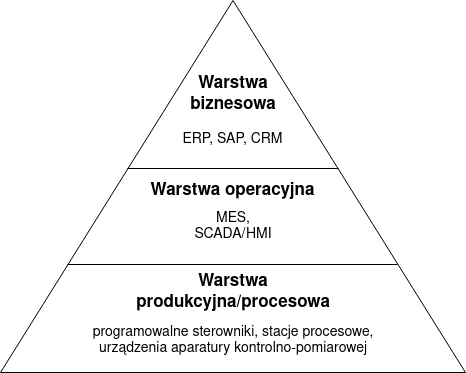
\includegraphics[scale=0.50]{piramida.png}
      \caption{Model piramidowy informatycznych systemów przemysłowych.}
      \label{fig:piramida}
\end{figure}

\subsection{Internet Rzeczy}\label{iot}

W podrozdziale przedstawiono przegląd definicji IoT oraz jego zastosowań, a także
opisano elementy tworzące IoT. Podrozdział zawiera też odniesienie do ważnego
w~kontekście omawianego zagadnienia przetwarzania w chmurze.

\subsubsection{Definicje i zastosowania Internetu Rzeczy}

\textbf{Internet Rzeczy} (ang. \emph{Internet of Things}, w skrócie: IoT) posiada różne definicje.
Jedną z prostszych jest: sieć przedmiotów z wbudowanymi czujnikami, które są podłączone
do Internetu \cite{intro-to-iot}. Bardziej szczegółowe jest ujęcie IoT jako sieci jednoznacznie
identyfikowalnych przedmiotów z wbudowanymi czujnikami, inteligencją obliczeniową
oraz powszechną łącznością z Internetem \cite{iot-hype-to-reality}.
Na nieco wyższym poziomie definiuje się IoT jako globalną infrastrukturę udostępniającą
zaawansowane usługi poprzez połączenie przedmiotów z wykorzystaniem technologii informacyjnych.
\cite{intro-to-iot}.

W każdej z przytoczonych
definicji zauważalne jest pewne podobieństwo pomiędzy IoT a CPS
scharakteryzowanym w rozdziale \ref{system-do-zbierania-danych}. Zagadnienia te
posiadają część wspólną, dotyczą podobnej tematyki (przede wszystkim połączenia świata fizycznego i logicznego),
lecz mają odrębną genezę i uwydatnia się w ich ramach różne aspekty:
inżynierię systemów sterowania w CPS oraz sieci i komunikację w IoT \cite{cps-vs-iot}.

Głównym zastosowaniem Internetu Rzeczy jest monitorowanie świata rzeczywistego
oraz wchodzenie z nim w interakcję, co może usprawnić działalność człowieka na wielu płaszczyznach.
Wśród praktycznych zastosowań IoT wymienia się między innymi:
sieci czujników i pomiary rozproszone, urządzenia (gadżety) ubieralne,
inteligentne budynki, miasta, logistyka, przemysł, a także marketing \cite{internet-reczy}.
Możliwości, jakie niesie IoT dla przemysłu zostały w sposób szczególny rozpatrzone
w rozdziale \ref{iiot}.

\subsubsection{``Rzeczy'' w IoT}

Wśród przedmiotów tworzących IoT wyróżnia się dwie kategorie:
\textbf{czujniki oraz urządzenia wykonawcze}. Są to odpowiedniki aparatury kontrolno-pomiarowej
wykorzystywanej w przemyśle (patrz: rozdział \ref{isp}). Czujniki umożliwiają
obserwację świata rzeczywistego i jej zapis w postaci cyfrowej.
Urządzenia wykonawcze są w stanie zmienić stan układu rzeczywistego
na podstawie otrzymanej informacji cyfrowej \cite{iot-hype-to-reality}.
Przykładowe czujniki to: przyciski, przełączniki, czujniki ruchu, czujniki gazów,
czujniki wibracji, czujniki temperatury, wilgoci,
nacisku, ultradźwięków i wielu innych wielkości fizycznych. Przykłady urządzeń
wykonawczych to: silniki, siłowniki liniowe, przekaźniki, zawory. Ważnym elementem
infrastruktury IoT są systemy wbudowane typu SoC (ang. \emph{System on a Chip}).
Są to układy elektroniczne, których poszczególne komponenty realizujące wymagane
funkcjonalności są zintegrowane w ramach jednego, kompletnego układu scalonego.
System typu SoC mogą zawierać m. in.: procesory lub mikrokontrolery, przetworniki
analogowo-cyfrowe i cyfrowo-analogowe, pamięci, procesory graficzne, interfejsy komunikacyjne \cite{intro-to-iot}, \cite{soc}.
Obok rozwiązań dedykowanych dużą popularnością cieszą się następujące platformy uniwersalne \cite{intro-to-iot}:
\begin{itemize}
      \itemsep0em
      \item Arduino --- Różne modele płytek rozwojowych wykorzystujące m. in. systemy
            SoC producenta Atmel oparte o mikrokontrolery AVR. Wśród zestawów płytek
            dostępne są moduły rozszerzeń posiadające przewodowe i bezprzewodowe interfejsy sieciowe.
      \item ESP --- Systemy typu SoC producenta Espressif Systems zawierające wbudowane
            bezprzewodowe interfejsy sieciowe.
      \item Raspberry Pi --- Zaawansowane płytki tworzące komputery jednopłtykowe (ang. \emph{single-board computer}).
            Można na nich uruchomić system operacyjny (również z interfejsem graficznym). Posiadają liczne
            interfejsy komunikacyjne (w tym sieciowe) \cite{rpi}.
\end{itemize}
Wymienione platformy uniwersalne mogą też stanowić pomost pomiędzy główną siecią w systemie
IoT (np. Ethernet lub WiFi) a innymi urządzeniami
peryferyjnemi komunikującymi się za pośrednictwem
uniwersalnych złącz pinowych GPIO albo interfejsów szeregowych, takich jak: SPI, I2C, RS232, USB \cite{intro-to-iot}.

\subsubsection{``Internet'' w IoT}

Wymiana informacji w systemach IoT może odbywać się w sposób przewodowy lub bezprzewodowy.
Stosowane modele komunikacji sieciowej bazują na standardowym modelu OSI bądź
internetowym stosie TCP/IP. W warstwie fizycznej i łącza danych
sieci IoT wykorzystuje się protokoły: Ethernet, WiFi, Bluetooth, sieci komórkowe,
ZigBee, Z-Wave, NFC. W warstwie sieciowej stosuje się: IPv4, IPv6 oraz zoptymalizowaną
pod IoT wersję IPv6 --- 6LoWPAN. Protokoły warstwy transportowej to m. in. TCP i UDP.
Warstwy sesji, prezentacji i aplikacji implementują powszechne używane internetowe protokoły, np.
HTTP, RTP, SMTP. Wśród protokołów najwyższych wastw opracowano również
protokoły dedykowane dla IoT --- są to m. in. MQTT i CoAP \cite{internet-reczy}, \cite{intro-to-iot}, \cite{iot-hype-to-reality}.


W sieciach IoT rozróżnia się trzy następujące modele komunikacyjne \cite{intro-to-iot}:

\begin{itemize}
      \itemsep0em
      \item Urządzenie -- Urządzenie (ang. \emph{Machine to Machine, Device to Device}, w skrócie: M2M)
            --- Urządzenia komunikują się pomiędzy sobą bez potrzeby translacji czy wykonywania
            skomplikowanego przetwarzania danych.
            W odniesieniu do zaprezentowanego w rozdziale \ref{isp} modelu piramidowego oznaczałoby to, że węzły
            działające w~ramach odrębnych warstw hierarchii mogłyby się ze sobą komunikować bezpośrednio, na tej samej płaszczyźnie;
      \item Urządzenie -- Brama (ang. \emph{Device to Gateway})
            --- Występuje, gdy zachodzi potrzeba translacji informacji wymienianej pomiędzy różnymi sieciami.
            Translacją zajmuje brama (ang. \emph{gateway}), którą tworzy dedykowane oprogramowanie i/lub urządzenie;
      \item Urządzenie -- Chmura (ang. \emph{Device to Cloud})
            --- Występuje, gdy zachodzi potrzeba zaawansowanego przetwarzania danych
            (statystyka, eksploracja danych, big data, składowanie, itp.),
            co nie jest możliwe w przypadku urządzeń o ograniczonych zasobach obliczeniowych,
            pamięciowych i energetycznych.
            Niektóre urządzenia są w stanie komunikować się z chmurą bezpośrednio, inne
            korzystają w tym celu z bram.
\end{itemize}

\subsubsection{Usługi chmurowe}

\textbf{Przetwarzanie w chmurze} (ang. \emph{cloud computing}) pozwala
na migrację części lub całości infrastruktury informatycznej do tzw. chmury.
W śród popularnych rozwiązań znajdują się:
Microsoft Azure, Amazon AWS, Google Cloud, czy IBM Cloud. Usługi chmurowe
udostępnianie przez wymienionych i wielu innych dostawców za pośrednictwem Internetu
noszą miano \textbf{chmury publicznej}.
Są one dostępne na życzenie i posiadają elastyczny
system rozliczeń, w którym koszta są zależne od faktycznie zużytych zasobów informatycznych
(cykle procesorów, pamięć, wykorzystanie łącza, liczba zapytań). Do zalet takiego
rozwiązania należą: łatwa skalowalność, konfigurowalność i duży wybór usług
ułatwiających utrzymanie infrastruktury informatycznej. Spośród wad należy wymienić
zależność od firm trzecich (dostawców chmury) oraz brak pełnej kontroli nad
posiadaną infrastrukturą. Niektóre firmy rozwijają też podobne, lecz dostępne
wyłącznie lokalnie, rozbudowane platformy infrastruktury informatycznej, zwane \textbf{chmurą prywatną}.
Tego typu rozwiązania są kosztowne, lecz dają pełną kontrolę nad posiadanymi zasobami \cite{iot-hype-to-reality}.

W ramach swoich usług dostawcy chmury udostępniają m.in.: przetwarzanie danych,
analitykę, eksplorację danych, uczenie maszynowe, konteneryzację, relacyjne i~nierelacyjne
bazy danych, integrację aplikacji, hosting aplikacji i stron internetowych,
maszyny wirtualne, narzędzia programistyczne, zarządzanie użytkwnikami, a~ponadto
platformy do zarządzania systemami IoT \cite{aws}, \cite{azure}.

Zarządzanie dużą ilością danych jest podstawowym zadaniem systemu IoT. Składa się ono
na: zbieranie, filtrowanie, agregację, przetwarzanie, składowanie, udostępnianie,
wizualizację oraz zabezpieczanie \cite{intro-to-iot}. Usługi chmurowe umożliwiają złożone zarządzanie
danymi oferując jednocześnie skalowalność, zdalny dostęp, opłaty zależne od zapotrzebowania
i gotowe rozwiązania programistyczne skracające czas rozwoju systemów
\cite{measuring-value-of-cloud-computing}, \cite{iot-and-cloud}, \cite{iot-in-industrial-sector}.

\subsection{Internet rzeczy w przemyśle}\label{iiot}

\textbf{Przemysłowym Internetem Rzeczy} (ang. \emph{Industrial Internet of Things}, w~skrócie: IIoT)
nazywamy rozwiązania IoT znajdujące zastosowanie w przemyśle. Do dziedziny
IIoT należą: komunikacja M2M oraz przemysłowe technologie komunikacyjne stosowane
w systemach automatyzacji. IIoT ma umożliwić lepsze zrozumienie procesów
przemysłowych, a w związku z tym zapewnić większą wydajność i zrównoważenie
produkcji. Innymi słowy, IIoT ma za zadanie ułatwić integrację \textbf{technologii operacyjnych}
(ang. \emph{Operation Technologies}, w skrócie: OT) oraz
\textbf{technologii informatycznych} (ang. \emph{Information Technologies}, w skrócie: IT)
\cite{iiot-challenges-opportunities-directions}.
Technologie operacyjne to systemy nadzorujące przebieg procesów przemysłowych,
zaś technologie informatyczne to systemy, których rolą jest jest gromadzenie
i przetwarzanie informacji wartościowych z perspektywy przedsiębiorstwa
\cite{ot-it-categorization-of-customer-concerns}.

Z zagadnieniem IIoT ściśle związane jest też pojęcie \textbf{Przemysłu 4.0} (ang. \emph{Industry 4.0})
reprezentujące czwartą rewolucję przemysłową. Jest to koncept stosunkowo uniwersalny
skupiający rozwiązania CPS, IoT, IIoT wykorzystywane w celu zwiększania efektywności
procesów przemysłowych w ramach tzw. inteligentnych fabryk (ang. \emph{smart factories})
\cite{iiot-cyber-manufacturing-systems}, \cite{iiot-challenges-opportunities-directions}.
Zależności pomiędzy wymienionymi pojęciami przedstawia rys.


Ze względu na konieczność funkcjonowania w specyficznym środowisku przemysłowym
IIoT posiada pewne cechy odróżniające od standardowego (konsumenckiego) IoT.
Wśród nich należy wymienić \cite{iiot-challenges-opportunities-directions}:
\begin{itemize}
      \itemsep0em
      \item Rozwój o charakterze ewolucyjnym, nie rewolucyjnym
            --- Podczas gdy wokół konsumenckiego IoT rozwijanych jest wiele nowych technologii i standardów,
            wdrażając systemy IIoT należy się liczyć z dużą bezwładnością
            przemysłowego środowiska technologicznego. Istnieje wiele sprawdzonych, dobrze
            funkcjonujących rozwiązań dedykowanych dla przemysłu \cite{isp};
      \item Infrastruktura komunikacyjna
            --- Infrastruktura IoT jest bardziej elastyczna, podczas gdy infrastruktura
            IIoT wymaga dostosowania do bardziej ustrukturyzowanych modeli komunikacyjnych;
      \item Ograniczenia
            --- W otoczeniu przemysłowym charakterystyczne są wysokie wymagania dotyczące
            ograniczeń czasowych (determinizmu), niezawodności, bezpieczeństwa danych oraz
            funkcjonowania w niesprzyjających warunkach środowiskowych.
\end{itemize}

Szczególną uwagę należy poświęcić stwierdzeniu, że \textbf{intencją wykorzystania IIoT nie
      jest zastąpienie tradycyjnych systemów automatyzacji procesów przemysłowych}.
Na tej płaszczyźnie istnieją bowiem dedykowane rozwiązania adresujące
problem ograniczeń spotykanych w automatyce przemysłowej.
Właściwym \textbf{celem wdrażania systemów IIoT jest zwiększanie wiedzy na temat procesów
      przemysłowych, co w efekcie pozwala na ulepszenie jego wydajności} \cite{iiot-challenges-opportunities-directions}.

Ze względu na tolerancję ograniczeń w systemie (m. in. opóźnień czasowych) można
wyróżnić trzy poziomy jakości usług komunikacyjnych \cite{iot-hype-to-reality}:
\begin{itemize}
      \itemsep0em
      \item Dostarczanie z wykorzystaniem najlepszych możliwości (ang. \emph{best effort})
            --- Komunikacja nie spełnia ścisłych ograniczeń czasowych, wykorzystywana jest
            maksymalna dostępna przepustowość. Jest to poziom jakości charakterystyczny
            dla usług internetowych;
      \item Dostarczanie w czasie gwarantowanym
            --- Komunikacja spełnia pewne ograniczenia czasowe, których niedotrzymanie
            skutkuje spadkiem korzyści płynących z~wykorzystawanych usług;
      \item Dostarczanie w czasie deterministycznym
            --- Komunikacja powinna spełniać ścisłe ograniczenia czasowe,
            których niedotrzymanie jest równoznaczne z awarią systemu.
\end{itemize}
Poziomy tolerancji opóźnień czasowych w różnych aplikacjach przedstawia rys. \ref{fig:tolerancja}

\begin{figure}
      \centering
      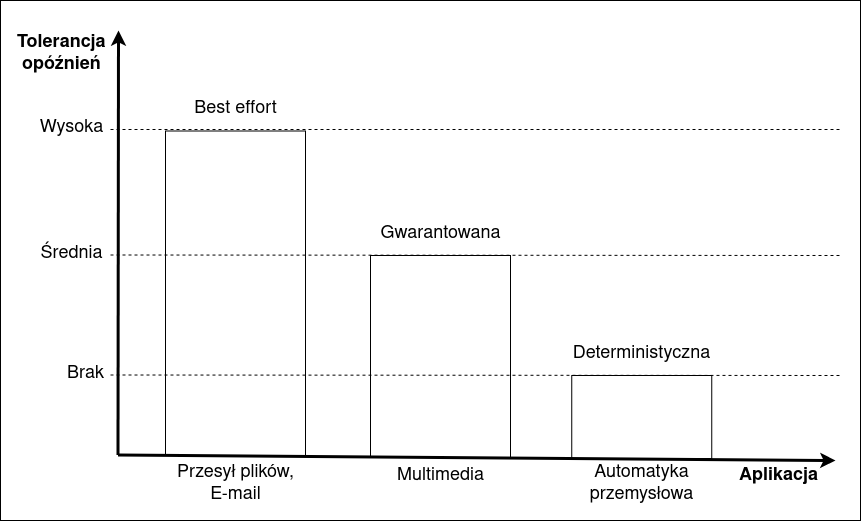
\includegraphics[scale=0.4]{tolerancja.png}
      \caption{Wykres przedstawiający poziomy tolerancji opóźnień dla różnych aplikacji.}
      \label{fig:tolerancja}
\end{figure}

Powszechna infrastruktura tworząca Internet, jak i usługi w nim dostępne, są z reguły
niedeterministyczne pod względem czasowym. Systemy IoT czy IIoT mogą więc
funkcjonować zgodnie paradygmatem \emph{best effort}. Aczkolwiek można wyobrazić
sobie pewien heterogeniczny system
IoT, w którym istnieje pewna sieć deterministyczna połączona z publicznym Internetem
za pomocą odpowiedniej bramy. Takie podejście może okazać się przydatne w przemyśle, gdzie
istnieje potrzeba integracji istniejących systemów automatyki z Internetem Rzeczy
\cite{iiot-design-and-impl-gateway}, \cite{iiot-rapid-integration-framework}.

W systemach IIoT popularny jest podstawowy, trójwarstwowy model architektury. Wśród jego
warstw wyróżniamy: warstwę brzegową (ang. \emph{edge}), warstwę platformową (ang. \emph{platform})
i warstwę biznesową (ang. \emph{enterprise}).
Model ten przedstawiono na rys.~\ref{fig:iiot-arch}. Do warstwy brzegowej należą
typowe urządzenia systemów automatyki przemysłowej, m.in. czujniki i urządzenia wykonawcze oraz
sterowniki (np. klasy PLC) oraz łączące je sieci komputerowe. Warstwa platformowa umożliwia zarządzanie
systemem IoT, akwizycję i agregację danych oraz ich trasowanie na wejścia
aplikacji i usług warstwy biznesowej, które
korzystają ze zgromadzonych danych w celu wspomagania
analityki, monitorowania, zarządzania, archiwizacji, itd. \cite{iiot-challenges-opportunities-directions},  \cite{models-innovative-iot}.

\begin{figure}
      \centering
      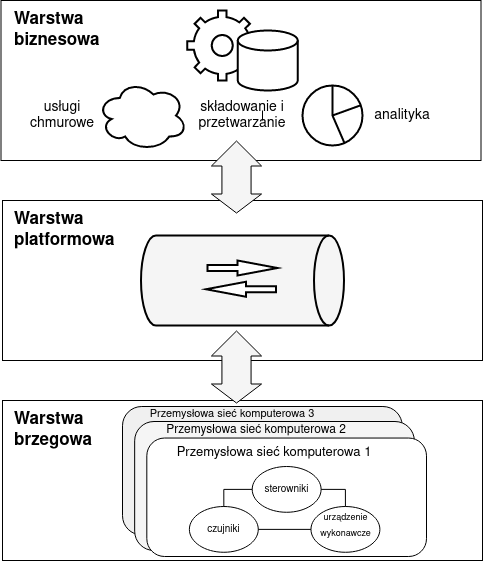
\includegraphics[scale=0.50]{iiot_arch.png}
      \caption{Model warstwowy systemów IIoT.}
      \label{fig:iiot-arch}
\end{figure}



\subsection{Ujęcie tematu w świetle zgromadzonych informacji}

Głównym zagadnieniem rozważanym
w ramach projektu jest zbieranie danych pomiarowych w środowisku
przemysłowym. Problem ten adresują technologie IIoT oraz usługi chmurowe.
Umożliwiają one gromadzenie i przetwarzanie danych w systemie rozproszonym składającym
się z szeroko pojętej aparatury kontrolno-pomiarowej (urządzeń cybernetyczno-fizycznych).
W niniejszej pracy podjęto zadanie \textbf{zaprojektowania architektury} opisanego systemu
oraz \textbf{realizacji jego prototypu}.

Sporządzenie koncepcji architektury systemu sprowadza się do wypracowania
\textbf{ogólnego rozwiązania} dla klasy zadań, jaką jest zbieranie danych w środowisku przemysłowym.
Zaproponowany model będzie więc abstrahować od konkretnych narzędzi, technologii,
urządzeń czy szczegółowych przypadków użycia. Przykładową implementację modelu ma
stanowić wykonany prototyp, na poziomie którego dobór technologii
i aparatury będzie skonkretyzowany na podstawie analizy i porównań dostępnych
narzędzi i usług informatycznych.

Modelem referencyjnym dla projektowanego systemu jest zaprezentowana w rozdziale
\ref{iiot} \textbf{trójwarstwowa architektura systemów IIoT}. Dla warstwy brzegowej przyjmuje
się, że w systemie jest zapewniony dostęp do dwóch rodzajów urządzeń: przemysłowe urządzenia
lub zespoły urządzeń aparatury kontrolno-pomiarowej pracujące w czasie rzeczywistym
w ramach sieci przemysłowej
(czujniki przemysłowe, wyspy czujników, moduły DAQ, moduły I/O, sterowniki, itp.)
oraz typowe dla IoT bezprzewodowe sieci sensorowe (ang. \emph{Wireless Sensor Networks}, w skrócie: WSN)
lub inne zespoły urządzeń zawierające czujniki komunikujące się z wykorzystaniem
interfejsów i protokołów charakterystycznych dla IoT \cite{iiot-gateway-introduction}
(przykłady takich urządzeń wymieniono w~rozdziale \ref{iot}). Implementację warstwy
platformowej realizują rozwiązania oferowane przez dostawców chmury.
Do warstwy biznesowej mogą należeć istniejące aplikacje
wspomagające działalność przedsiębiorstwa
(m. in. systemy klasy ERP) oraz mogące przejmować ich funkcje usługi chmurowe.
Pewną lukę, element brakujący w proponowanym modelu stanowi konieczność dopasowania
do różnych protokołów sieci przemysłowych i IoT. Istnieje również potrzeba integracji
warstwy brzegowej i platformowej zaproponowanego modelu. Są to krytyczne zadania
przypisywane systemom IIoT. Do rozwiązania
przytoczonego problemu stosuje się tzw. \textbf{bramy IoT} (ang. \emph{IoT gateways}). Są to zwykle
urządzenia wraz z~oprogramowaniem będące w stanie integrować zarówno protokoły
warstwy fizycznej i łącza danych, jak i dokonywać translacji protokołów wyższych warstw
(tzw. bramy semantyczne) wraz z możliwością udostępniania danych za pośrednictwem
Internetu \cite{iiot-heterogenous-gateways}. Bramy mogą realizować ponadto
wstępne przetwarzanie danych odciążając w ten sposób usługi wyższych warstw.
Jest to tzw. koncepcja \textbf{przetwarzania brzegowego} (ang. \emph{edge computing}) \cite{iot-gateway-medical-and-industrial}.
W ogólniejszym rozumieniu bramy IoT mają stanowić pomost pomiędzy technologią operacyjną a
technologią informatyczną \cite{iiot-gateway-introduction}, \cite{iiot-challenges-opportunities-directions}.

Otrzymano zatem podstawowy zarys projektowanego systemu.
Składa się on z~urządzeń pomiarowych udostępniających dane w ramach sieci
przemysłowych oraz IoT. Integracji różnych urządzeń i wstępnego przetwarzania
dokonuje dedykowana brama (bramy) IoT. Przekazuje ona dane w spójnym, jednolitym
formacie do usług chmurowych i innych aplikacji za pośrednictwem Internetu.
Te z kolei mogą realizować zaawansowane przetwarzanie, składowanie, udostępnianie
i wizualizację danych.

Wśród istniejących, komercyjnych rozwiązań o podobnej dziedzinie funkcjonalnej
znaleziono następujące przykłady:
\begin{itemize}
      \itemsep0em
      \item Sensemetrics --- Rozwiązanie amerykańskiej firmy Industrial IoT Solutions
            oparte na standaryzowanej architekturze warstwowej. Jest to system do akwizycji
            i zarządzania danych. Producent przypisuje swojemu systemowi wysoką konfigurowalność \cite{sensmetrics};
      \item Nazca 4.0 --- System rozwijany przez polską firmę APA Group zorientowany na Przemysł 4.0.
            Wśród użytych technologii producent wymienia IoT, inteligentne czujniki,
            przetwarzanie w chmurze, integrację systemów \cite{nazca};
      \item IXON --- Kompletne rozwiązanie IIoT holenderskiej firmy o tej samej nazwie.
            System składa się z platformy internetowej umożliwiającej nadzór, analitykę i~wizualizację danych,
            a~także dedykowanego routera/bramy IoT. Urządzenie wraz z~oprogramowaniem
            integruje takie systemy i protokoły jak: OPC UA, Modbus, Ethernet \cite{ixon}.
\end{itemize}


\section{Specyfikacja wymagań}\label{wymagania}

W niniejszym rozdziale przedstawiono szczegółową specyfikację wymagań
stawianych wobec projektowanego systemu i prototypu. Dokumentacja składa się
z wymagań funkcjonalnych i niefunkcjonalnych, przypadków użycia oraz scenariuszy
biznesowych implementowanych w ramach prototypu.

\subsection{Wymagania funkcjonalne}

Do założonych ogólnych funkcjonalności systemu należą: zbieranie, przetwarzanie,
składowanie, udostępnianie i wizualizacja danych pomiarowych. W kolejnych
podrozdziałach opisano szerzej każde z wymienionych wymagań wraz z nadaniem kontekstu
użycia.

\subsubsection{Zbieranie danych pomiarowych}

Zbieranie (gromadzenie) danych pomiarowych to podstawowe zadanie projektowanego systemu.
Pod pojęciem ``dane pomiarowe'' rozumie się opis obiektów i zjawisk fizycznych
zapisany w postaci cyfrowej, który jest zwykle przyporządkowany do określonego
punktu lub przedziału w czasie. Ciąg takich opisów nazywa się szeregiem czasowym \cite{time-series}.
Do możliwych źródeł danych pomiarowych należą: aparatura pomiarowa (czujniki, sensory),
pamięć masowa, użytkownicy wchodzący w~interakcję z systemem oraz inne systemy informatyczne.
Projektowany system powinien \textbf{udostępniać interfejs wejściowy} umożliwiający zbieranie
i przekazywanie danych pochodzących z~wymienionych źródeł. Należy ponadto uwzględnić
fakt, że urządzenia dostarczające dane mogą komunikować się na różne sposoby.
Stąd konieczne jest, aby system był przystosowany do współpracy z popularnymi
interfejsami oraz protokołami komunikacyjnymi.

\subsubsection{Przetwarzanie danych}

Przetwarzanie danych (ang. \emph{data processing}) to przekształcanie danych
wejściowych z użyciem komputerów dla uzyskania informacji
wartościowych w określonym kontekście. Korzyści wynikające z przetwarzania
danych wykorzystuje się w prowadzeniu organizacji lub przedsiębiorstw \cite{data-processing}.
Przetwarzanie jest oczywistym następstwem zbierania danych. Realizowany
system ma więc za zadanie umożliwić \textbf{przetwarzanie zgromadzonych danych pomiarowych}
--- zarówno na poziomie sprzętowym, jak i~programowym. Wśród możliwych przykładów
przetwarzania danych w systemie można wymienić: agregację danych
(scalanie wyników, wyznaczanie statystyk),
obliczanie kluczowych wskaźników efektywności prowadzonej działalności
(ang. \emph{Key Performance Indicators}, w skrócie: KPI), uczenie maszynowe
(zadania klasyfikacji, prognozowanie, optymalizacja procesów), automatyzację zadań.

\subsubsection{Składowanie danych}

Z przetwarzaniem danych ściśle związany jest problem ich składowania.
W ramach dziedziny biznesowej istnieje zwykle potrzeba przyszłego wykorzystania
zebranych danych oraz wyników ich przetwarzania. Trwały zapis danych dokumentuje
procesy zachodzące w przedsiębiorstwie i udogadnia sprawowanie kontroli; pozwala
na gromadzenie większej ich ilości i w konsekwencji pogłębioną, bardziej dokładną
analizę. Zatem oczekuje się, aby projektowany system \textbf{realizował również
      funkcjonalność składowania (archiwizacji) danych pomiarowych w bazach danych}
i umożliwiał dostęp do nich w przyszłości.

\subsubsection{Wizualizacja danych}

Aby gromadzenie i przetwarzanie danych pomiarowych mogło przynieść jakiekolwiek
korzyści dla przedsiębiorstwa niezbędne jest, aby dane otrzymywane na wyjściu realizowanego
systemu posiadały reprezentację interpretowalną, łatwo przyswajalną dla człowieka.
Możliwe jest wówczas dokonywanie dalszej analizy i zadań obserwacji, monitorowania
czy zarządzania. System \textbf{powinien zatem udostępniać przyjazny dla człowieka
      interfejs (graficzny)}, w którym dane przedstawione są za pomocą tabel, wykresów,
diagramów, plików o przejrzystej strukturze.

\subsubsection{Udostępnianie danych}

Z efektów działania projektowanego systemu bezpośrednio mogą korzystać nie tylko
ludzie, lecz także inne systemy. Systemy informatyczne wspomagające funkcjonowanie
pojedynczych, jak również współpracę wielu przedsiębiorstw zwykle nie stanowią
rozwiązań jednolitych, lecz tworzą rozproszony system mniej lub bardziej
powiązanych aplikacji i urządzeń. Wymaga się więc, aby realizowany system \textbf{mógł udostępniać
      zgromadzone dane i wyniki ich przetwarzania na potrzeby innych systemów (klientów)},
które realizują kolejne etapy przetwarzania danych.

\subsection{Wymagania niefunkcjonalne}

Rozdział zawiera opis następujących wymagań niefunkcjonalnych:
wykorzystanie technologii IoT i przetwarzania w chmurze, dostosowanie do środowiska
przemysłowego, ogólność rozwiązania, skalowalność i bezpieczeństwo danych. Szczegółowe
rozważania dotyczące wymienionych założeń przedstawiono w ramach kolejnych
podrozdziałów.

\subsubsection{Wykorzystanie technologii IoT i przetwarzania w chmurze}

Wykorzystanie Internetu Rzeczy to podstawowe założenie, które zostało ujęte
w~temacie niniejszej pracy i zaznaczone przy określeniu
celu projektu. Do najważniejszych zastosowań IoT należy zbieranie dużej ilości
danych z wielu różnych urządzeń. Użycie rozwiązań z tej dziedziny jest więc wyborem uzasadnionym.
Zadaniem krytycznym w systemach IoT jest przetwarzanie zebranych danych.
Problem ten podejmują przede wszystkim oferowane za pośrednictwem Internetu
usługi chmurowe. Tak więc Internet Rzeczy i~przetwarzanie w~chmurze w~stopniu
znaczącym odpowiadają na większość wymagań funkcjonalnych przedstawionych w~poprzednim rozdziale.

Użycie technologii IoT
w realizowanej pracy sprowadza się do zastosowania odpowiednich modeli komunikacyjnych,
sieci, protokołów oraz urządzeń. Wykorzystanie chmury obliczeniowej polega
na wyborze usług wspomagających zarządzanie urządzeniami IoT,
a także udogadniających gromadzenie, przetwarzanie, składowanie i udostępnianie
danych.

\subsubsection{Dostosowanie do środowiska przemysłowego}

Drugim założeniem podstawowym obejmującym zakres niniejszej pracy
jest \textbf{przystosowanie projektowanego systemu do zastosowania w przemyśle.}
W wielu przedsiębiorstwach istnieją już sprawdzone systemy automatyki wyposażone
w aparaturę pomiarową. Jako że rozwój technologiczny w przemyśle ma z reguły
charakter stopniowy, wymaga się, aby projektowany system \textbf{integrował się
      z obecnie funkcjonującymi systemami}, co oznacza konieczność posiadania
odpowiednich interfejsów komunikacyjnych i implementowania określonych protokołów
charakterystycznych dla rozproszonych systemów przemysłowych.

Jak już wspomniano w rozdziale \ref{analiza}, systemy nadzorujące
procesy przemysłowe muszą zwykle działać w ramach twardych ograniczeń czasowych.
Natomiast wykorzystanie technologii internetowych gwarantuje działanie na poziomie
\emph{best effort}. Celem ich stosowania w przemyśle nie jest jednak zastąpienie
istniejących systemów automatyki, lecz ich integracja z systemami warstwy IT,
które niekoniecznie operują w sztywnych ramach czasowych.
Aczkolwiek, żeby zapewnić szerszą współpracę projektowanego systemu
z istniejącymi rozwiązaniami przemysłowymi, należy \textbf{uwzględnić możliwość jego funkcjonowania
      w czasie rzeczywistym na poziomie lokalnym}, tzn. w ramach warstwy brzegowej
(patrz: rozdział \ref{analiza}, rys. \ref{fig:iiot-arch}).

W środowisku przemysłowym oczekuje się zwiększonej niezawodności systemów
zarówno na poziomie sprzętowym, jak i programowym. Choć w przypadku IIoT nie jest
to zwykle wymaganie o stopniu tak krytycznym, jak w standardowych systemach automatyki,
to w projekcie systemu należy uwzględnić w zakresie podstawowym
zagadnienia \textbf{redundancji, diagnostyki i możliwości funkcjonowania w niesprzyjających
      warunkach środowiskowych}.

\subsubsection{Ogólność rozwiązania}

Pożądaną cechą projektowanego systemu jest jego uniwersalność. Wypracowane rozwiązanie
powinno być możliwie niezależne od specyficznych urządzeń, narzędzi technicznych,
oprogramowania, czy dostawców chmury. Takie podejście pozwala na implementację różnych przypadków biznesowych
oraz dostosowanie do istniejącej w przedsiębiorstwach infrastruktury sprzętu i oprogramowania
z uwzględnieniem indywidualnych preferencji, wymagań i posiadanych zasobów.

Integrację różnych systemów informatycznych na odpowiednich poziomach abstrakcji
zapewniają sieci komputerowe, interfejsy i protokoły.
Stąd \textbf{kluczowym aspektem projektowanego systemu --- co już kilkukrotnie zostało podkreślone ---
      jest dostarczenie wsparcia dla popularnych
      interfejsów, protokołów i modeli wymiany informacji stosowanych w~IoT, przemyśle oraz
      aplikacjach internetowych i usługach chmurowych}. Wśród rozwiązań sieciowych
należy w szczególności uwzględnić: Ethernet (również klasy RTE szeroko stosowany
w przemyśle \cite{isp}), sieci i standardy komunikacji bezprzewodowej (WiFi, Zigbee, Z-Wave, Bluetooth, GSM).
Wiele urządzeń wbudowanych (w tym przemysłowych) komunikuje się za pośrednictwem
interfejsów szeregowych: RS232/485, USB, SPI, I2C. Spośród protokołów należy
wziąć pod uwagę MQTT i CoAP, które są dedykowane dla rozwiązań IoT. Aplikacje
internetowe wykorzystują obecnie najczęściej protokół HTTP. W przemyśle
stosuje się powszechnie protokół Modbus/TCP, a także zapewniające determinizm czasowy
protokoły dedykowane dla sieci Ethernet: Profinet, EtherCAT, Ethernet Powerlink.
Warty uwzględnienia jest też przemysłowy model wymiany informacji OPC~UA.

Wraz z implementacją popularnych protokołów wymagane jest ponadto \textbf{zapewnienie
      jednolitego formatu danych na poziomie warstwy aplikacji}, który ma zagwarantować przenośność,
łatwą wymianę danych pomiędzy współpracującymi systemami. Formaty
te powinny być uprzednio specyfikowane, a projektowany system powinien być do
nich zaadaptowany --- analogicznie, jak w przypadku protokołów.

Obok przystosowania do różnych sposobów komunikacji ważnym kryterium uniwersalności
systemu jest elastyczność oprogramowania.
W systemie, w którym zbierane są dane z wielu różnych urządzeń, wymagania dotyczące
ich przetwarzania podlegają częstej zmianie i ewolucji. Mogą się one również
zasadniczo różnić pomiędzy poszczególnymi przedsiębiorstwami. \textbf{Oczekuje się zatem,
      aby system umożliwiał łatwą modyfikację i rozbudowę realizowanej logiki, jak
      również wymianę komponentów}. Ponadto należy uwzględnić fakt, że w zarządzaniu
systemem przemysłowym niekoniecznie muszą uczestniczyć zawodowi programiści,
z czym wiąże się potrzeba, aby \textbf{model programistyczny systemu był zrozumiały
      także dla specjalistów innych dziedzin techniki i analityków}.

Poza wypracowaniem ogólnej specyfikacji projektu wymaga się
również \textbf{wykonania prototypu, którego celem jest weryfikacja przedstawionej koncepcji}.
Na jego potrzeby mają zostać zaimplementowane określone scenariusze
biznesowe z wykorzystaniem wybranych urządzeń, sposobów komunikacji, narzędzi i
usług chmurowych.

\subsubsection{Skalowalność}

Projekt powinien przewidywać możliwość zmiany skali infrastruktury przedsiębiorstwa,
w ramach której ma on być wdrożony. Wymaga się, aby system mógł być
w~stosunkowo prosty, szybki i tani sposób zaadaptowany do nowych warunków pracy,
które są rezultatem zmieniającej się liczby obsługiwanych
urządzeń i~ilości koniecznych do przetworzenia danych. Dostosowanie systemu sprowadza
się w głównej mierze do przydzielenia odpowiednich zasobów sprzętowych i programowych.

\subsubsection{Bezpieczeństwo danych}

Wymaganiem stawianym wobec większości systemów informatycznych jest bezpieczeństwo
danych. Również w środowisku przemysłowym przetwarzane dane są zwykle traktowane
jako poufne, zaś ograniczenie dostępu do systemów sterowania ma charakter krytyczny,
gdyż mają one realny wpływ na bezpieczeństwo zasobów przedsiębiorstwa~--- w tym także
i ludzi. W ramach projektu należy rozważyć w zakresie podstawowym kwestie
bezpieczeństwa w aspekcie autoryzacji dostępu do systemu (w świecie rzeczywistym oraz
cyfrowym), a także zapewnienia poufności z wykorzystaniem szyfrowania i
metod ochrony przed kradzieżą.

\subsection{Przypadki użycia}

Ogólne ujęcie funkcjonalności projektowanego systemu z perspektywy użytkowników,
zewnętrznych urządzeń i systemów modeluje diagram przypadków użycia przedstawiony
na rys. \ref{fig:use-case}. Na jego potrzeby zdefiniowano abstrakcyjne
źródło danych, które może stanowić aparatura pomiarowa, sterowniki przemysłowe, komputery,
urządzenia wbudowane, pamięć masowa, a także inne systemy. Źródło przesyła
dane do systemu, który dokonuje ich konwersji na pożądany format i umożliwia
dalsze składowanie, przetwarzanie, udostępnianie i wizualizację. Dane są
udostępniane na potrzeby innych systemów informatycznych (aplikacji klienckich).
Są one także bezpośrednio prezentowane pracownikom obsługi procesu przemysłowego
i analitykom w ramach wizualizacji. Wymienieni pracownicy we
współpracy z programistami i testerami uczestniczą
w procesie implementacji, modyfikacji i rozbudowy logiki przetwarzania danych.
Administrator systemu zajmuje się jego konfiguracją i utrzymaniem
poszczególnych jego komponentów. Praca ta polega na
instalacji urządzeń warstwy sprzętowej, zarządzaniu
użytkownikami i dostępem do systemu, integracji poszczególnych jego komponentów,
ustawieniu parametrów połączeń sieciowych i protokołów, monitorowaniu
i usuwaniu awarii.

\begin{figure}
      \centering
      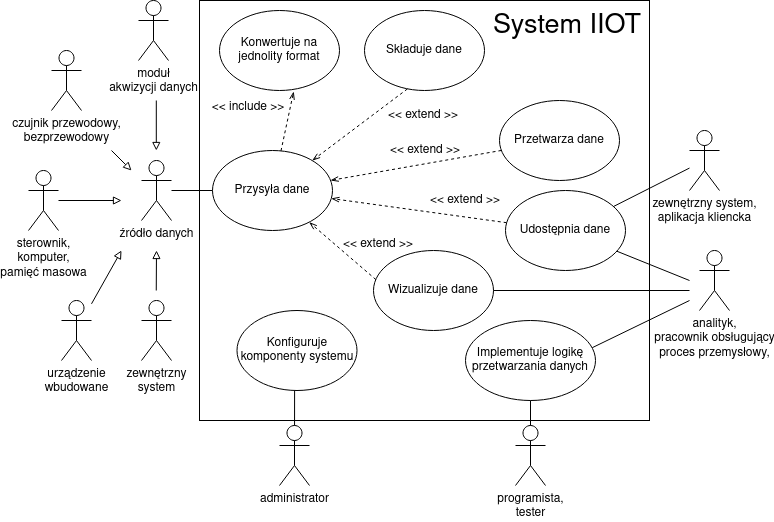
\includegraphics[width=\textwidth]{use-case.png}
      \caption{Diagram przypadków użycia systemu.}
      \label{fig:use-case}
\end{figure}

\subsection{Scenariusze wykorzystania systemu}\label{scenariusze}

Na potrzeby walidacji funkcjonalności realizowanego projektu dokonano wyboru przykładowych
scenariuszy biznesowych, które mają zostać zaimplementowane przez prototyp.
Przyjęto założenie, że w środowisku docelowym w obrębie lokalnej sieci
są zainstalowane urządzenia pomiarowe, które komunikują się odpowiednio
z wykorzystaniem protokołów
MQTT, CoAP oraz Modbus/TCP. Pierwsze dwa są charakterystyczne dla IoT, natomiast
ostatni jest popularny wśród rozwiązań przemysłowych. System ma za zadanie
integrować się z lokalną siecią i wymienionymi protokołami, z użyciem
których gromadzone będą dane. Te z kolei mają zostać skonwertowane na oczekiwany,
jednolity format warstwy aplikacji i przekazane do usług chmurowych, gdzie odbywa się dalsze
przetwarzanie i składowanie. System powinien także umożliwić przeglądanie danych
w bazie oraz podstawową wizualizację za pośrednictwem wykresów, diagramów, tabel.
Szczegółowy opis przyjętych scenariuszy biznesowych przedstawiono w kolejnych
podrozdziałach.

\subsubsection{Monitorowanie parametrów powietrza}

W określonych pomieszczeniach zakładu produkcyjnego zainstalowano sieć bezprzewodowych
czujników temperatury i wilgoci WiFi, która jest połączona z siecią lokalną.
Czujniki potrafią komunikować się z wykorzystaniem protokołu MQTT/TCP. Do monitorowanych
pomieszczeń należą: chłodnia, magazyn i hala produkcyjna. Prototyp systemu ma za zadanie
zbierać, składować, udostępniać i wizualizować zmierzone parametry powietrza.

\subsubsection{Monitorowanie stanu zużycia chemii przemysłowej}

W zakładzie produkcyjnym rozlokowane są trzy zbiorniki (bufory) chemii przemysłowej.
Zbiorniki są połączone z zewnętrznym zbiornikiem głównym, z którego uzupełniany
jest ich stan. W celu automatycznego napełniania zbiorników wykorzystano sterownik
klasy PLC podłączony do lokalnej sieci Profinet, który otwiera albo zamyka
odpowiednie zawory i nadzoruje pracę pomp.
Odczytuje on dane z przepływomierzy pozwalające na monitorowanie stanu
zużycia chemii w każdej z trzech stref oraz poziom cieczy w zbiorniku głównym.
Zadaniem prototypu jest cykliczny odczyt wskazań dla każdego
zbiornika znajdujących się w pamięci PLC z wykorzystaniem protokołu Modbus/TCP.
Zebrane dane powinny być składowane w chmurze oraz wizualizowane.

\subsubsection{Wyznaczanie parametru KPI}

Na wyjściu trzech linii procesowych rozmieszczona jest aparatura przeznaczona
do oceny jakości dostarczanych produktów. Może ją stanowić zaawansowane
rozwiązanie wykorzystujące specjalizowane przyrządy pomiarowe i sztuczną inteligencję lub
pracownik dokonujący oceny manualnie i wpisujący wyniki do komputera. Urządzenie,
w którym zapisywany jest wynik, jest podłączone do lokalnej sieci Profinet.
Informacja o spełnieniu albo niespełnieniu wymagań jakościowych jest przesyłana
do serwera z~wykorzystaniem CoAP/UDP w oparciu o architekturę REST. Zadaniem
realizowanym przez prototyp jest odbiór przesyłanych rezultatów inspekcji
(implementacja serwera), przetwarzanie i składowanie w chmurze. Przetwarzanie
danych polega w tym przypadku na wyznaczaniu wartości parametru FTQ
(ang. \emph{First Time Quality}). Jest to jeden ze wskaźników KPI będący miarą
zdolności linii do produkowania bez wad. FTQ to iloraz liczby produktów,
które spełniły wymagania jakościowe i liczby wszystkich dostarczonych produktów
wyrażony wzorem \eqref{eq:ftq}.
Jego wartość podaje się zwykle w procentach \cite{isp}. Wskaźnik FTQ
wyznaczany dla każdej z trzech rozpatrywanych linii procesowych powinien być na bieżąco wizualizowany.

\begin{equation}
      FTQ = \frac{s}{n}\label{eq:ftq}
\end{equation}
\noindent gdzie: \\
$s$ --- liczba produktów wyprodukowanych bez wad,\\
$n$ --- liczba wszystkich produktów wyprodukowanych w procesie.

\begin{figure}[h]
      \centering
      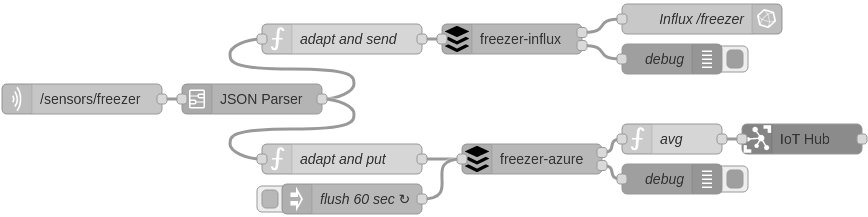
\includegraphics[width=\textwidth]{flow1.png}
      \caption{Model piramidowy informatycznych systemów przemysłowych.}
      \label{fig:flow1}
\end{figure}

\begin{figure}[h]
      \centering
      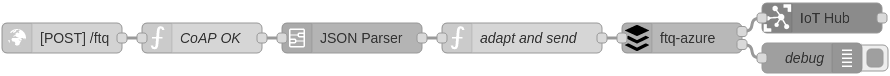
\includegraphics[width=\textwidth]{flow2.png}
      \caption{Model piramidowy informatycznych systemów przemysłowych.}
      \label{fig:flow2}
\end{figure}

\begin{figure}[h]
      \centering
      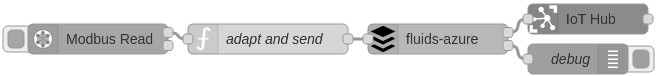
\includegraphics[width=0.75\textwidth]{flow3.png}
      \caption{Model piramidowy informatycznych systemów przemysłowych.}
      \label{fig:flow3}
\end{figure}



\section{Specyfikacja wewnętrzna}\label{spec-zew}

\subsection{Ogólna koncepcja rozwiązania}\label{ogolna-koncepcja}

Proponowane rozwiązanie opiera się na trójwarstwowym modelu architektury
systemów IIoT (patrz: rozdział \ref{iiot}, rys. \ref{fig:iiot-arch}), który
zaadaptowano w celu praktycznego zastosowania, uwzględniwszy zdefiniowane
wymagania projektowe oraz dostępne narzędzia i usługi. Wypracowaną koncepcję
zobrazowano na rys. \todo{dodać rysunek}.

Pierwszym punktem zbierania danych w systemie
są bramy IoT (IIoT). Ich wykorzystanie
pozwala na integrację zróżnicowanej pod względem technicznym aparatury pomiarowej.
Bramy mają dostarczać odpowiednie interfejsy fizyczne, jak również dokonywać
translacji protokołów pośrednicząc w ten sposób w wymianie danych
pomiędzy warstwą brzegową i biznesową \cite{iiot-gateway-introduction},
\cite{iiot-heterogenous-gateways}, \cite{iot-gateway-medical-and-industrial},
\cite{modbus-iot-gateway}, \cite{iiot-design-and-impl-gateway}. Realizują one także
wstępne przetwarzanie w warstwie brzegowej (ang. \emph{edge computing}) i ułatwiają
sprawowanie kontroli nad przepływem danych w systemie \cite{iiot-architecture-and-gateway}.
Idea stosowania bramy IoT w przemyśle umożliwia
spełnienie głównego zadania IIoT, jakim jest połączenie technologii operacyjnych
i technologii informacyjnych (ang. \emph{OT/IT convergence}) \cite{iiot-opensource-gateway}.
Na omawianym rysunku zamieszczono trzy bramy, które integrują urządzenia odpowiednio
w ramach sieci bezprzewodowej, przemysłowej sieci Ethernet oraz interfejsów szeregowych.
Jest to podział poglądowy. W zależności od indywidualnych potrzeb i dostępnego sprzętu możliwe są różne
konfiguracje: pojedyncza brama pracująca w wielu sieciach, bramy dedykowane
dla określonych sieci, hierarchiczna struktura bram.

Za pośrednictwem Internetu brama
przekazuje dane do warstw wyższych, z wykorzystaniem których odbywa się kolejny etap gromadzenia,
a także przetwarzanie, składowanie i udostępnianie danych. Są to warstwy platformowa
i biznesowa, których techniczną implementację oferują odpowiednie usługi chmurowe
popularnych dostawców: Microsoft, Amazon, Google, Intel, IBM. Możliwe jest też
wdrożenie przez przedsiębiorstwo chmury prywatnej lub dedykowanej infrastruktury
i oprogramowania.

Do warstwy biznesowej należą także aplikacje klienckie, którym dane składowane
w bazie są udostępniane za pośrednictwem protokołów
internetowych, np. HTTP, AMQP, MQTT. Wśród potencjalnych klientów należy wyróżnić
oprogramowanie, które będzie realizowało zdefiniowane w ramach projektu wymaganie wizualizacji
danych.

\subsection{Komponentowy model architektury}

Wychodząc od koncepcji opisanej w poprzednim rozdziale opracowano
formalny model architektury projektowanego systemu przedstawiony
w postaci diagramu na rys. \todo{usupełnić}. Składa się on z licznych luźno
powiązanych komponentów rozlokowanych na określonych platformach sprzętu i oprogramowania.
Rozdział systemu na pojedyncze elementy składowe odpowiada na wymaganie uniwersalności, zapewnia
lepszą konfigurowalność i skalowalności. Modularny charakter systemu
udogadnia także niezależną modyfikację i rozbudowę poszczególnych podzespołów.
Komponenty podlegają swobodnej wymianie
i zwielokrotnieniu pod warunkiem spełnienia wymaganego interfejsu.
Biorąc pod uwagę fakt, że system obejmuje szeroką dziedzinę (od warstwy procesowej
po wysokopoziomowe aplikacje IT) i może być utrzymywany przez zespoły o różnych
specjalnościach, jest to aspekt szczególnie ważny. Podstawą współpracy
grup komponentów osadzonych \texttt{Bramie IIoT}, \texttt{Chmurze} i na 
\texttt{Urządzeniach Klienckich} jest
Internet i popularne protokoły internetowe: HTTP, FTP, MQTT, AMQP, WebSocket, TLS.

Zamieszczona na omawianym diagramie \texttt{Brama IIoT} to urządzenie (system komputerowy)
posiadające odpowiednie porty (interfejsy fizyczne, porty sieciowe, porty szeregowe),
przez które może komunikować się z aparaturą pomiarową reprezentowaną przez
\texttt{Źródło danych}. Zbieranie danych w jednym miejscu, translację protokołów,
przetwarzanie brzegowe i komunikację z komponentami udostępnianymi za pośrednictwem
Internetu realizuje dedykowane \texttt{Oprogramowanie}.
Jest to komponent złożony składający z \texttt{Komponentów Przetwarzania Brzegowego}
realizujących określone funkcje przetwarzające oraz \texttt{Buforów Brzegowych},
które umożliwiają agregację i zachowanie jednolitego formatu danych wyjściowych.
Szczegóły komponentu \texttt{Oprogramowania}
przedstawiono na rys. \todo{dodać rys}
W ramach bramy może funkcjonować również sprzętowo-programowy moduł
czasu rzeczywistego RT (ang. \emph{Real-Time}), którego celem jest współpraca
z lokalnym systemem czasu rzeczywistego. W systemie przewiduje się istnienie wielu źródeł
danych, jak i możliwe jest wykorzystanie wielu bram. Ponadto żeby zapewnić większą niezawodność i skalowalność
można rozważyć budowę klastra bram z redundancją i równoważeniem obciążenia.
Jako sprzętową realizację bramy w literaturze spotyka się komputer jednopłytkowy
RaspberryPi, a także bramki z serii Siemens Simatic IOT2000
\cite{iiot-opensource-gateway}, \cite{design-impl-node-gateway},
\cite{low-cost-esp32-pi-node-red-scada}, \cite{modbus-iot-gateway}. Można też
wziąć pod uwagę wykorzystanie platformy BeagleBone Black, czy dedykowanych rozwiązań
producentów Cisco, Dell, Huawei, Hewlett Packard, NXP i innych \cite{gateways}.
Do realizacji oprogramowania można posłużyć się narzędziami przeznaczonymi do
integracji urządzeń IoT. Jednym z najpopularniejszych programów jest
Node-RED \cite{testing-node-red}, \cite{flow-programming}, \cite{iot-gateway-medical-and-industrial},
\cite{design-impl-node-gateway}, \cite{iiot-opensource-gateway}, \cite{low-cost-esp32-pi-node-red-scada}.
Jest to darmowe narzędzie \emph{open source} działające w środowisku Node.js na
systemach Linux, Windows. Alternatywne darmowe rozwiązania to m.in. n8n.io, Total.js Flow.
Wśród ofert komercyjnych dostępne są przykładowo platformy Crosser, Bosch ProSyst
\cite{node-red}, \cite{n8n}, \cite{total-js-flow}, \cite{crosser}, \cite{gateways}.

Przedstawiony na rys. \todo{dodać rys} diagram o nazwie \texttt{Chmura}
może w rzeczywistości odpowiadać chmurze publicznej, prywatnej lub innej
dedykowanej infrastrukturze sprzętu i oprogramowania. W niniejszym projekcie
w szczególności rozpatruje się wariant z chmurą publiczną, której usługi są dostępne
za pośrednictwem Internetu. Pozwalają one na techniczną realizację postawionych
wymagań przetwarzania, składowania i udostępniania danych.
Umieszczone wewnątrz diagramu komponenty zostały dobrane
pod kątem zdefiniowanych wymagań funkcjonalnych. \texttt{Platforma IoT}
to komponent, który odbiera dane przychodzące z urządzeń (bram IIoT).
Umożliwia również zarządzanie urządzeniami:
dodawanie, usuwanie, modyfikację uprawnień, a także monitoring i diagnostykę.
Dane z platformy mogą zostać bezpośrednio składowane w \texttt{Bazie Danych}.
Możliwe jest też przekazanie ich na wejście \texttt{Komponentu Przetwarzającego}.
Pod tym pojęciem rozumiane są wszelkie usługi chmurowe realizujące tzw. bezserwerowe
przetwarzanie danych (ang. \emph{serverless computing}). Nie oznacza to, że
serwer nie istnieje, lecz że jest on niejako ,,zakryty'' przed programistą, który skupia
się jedynie na dostarczeniu logiki w postaci wsadowej \cite{azure-serverless}.
Usługi przetwarzania bezserwerowego dokonują ewentualnego odczytu i zapisu do \texttt{Bazy Danych}. 
Wśród usług oferowanych przez liderów rynku chmurowego 
--- Amazon Web Services (AWS) i Microsoft Azure \cite{gartner-cloud-liders}
--- dokonano przeglądu przykładowych, które mogą być użyte do implementacji opisanych komponentów.
W poniższych punktach oddzielono znakiem ,, | '' odpowiednio nazwy usług AWS i Azure,
które mają podobny zakres funkcjonalny \cite{azure-aws-comparison}.\\

\noindent\textbf{Przykładowe usługi użyteczne do realizacji \texttt{Platformy IoT}}:
\begin{itemize}
      \itemsep0em
      \item IoT | IoT Hub ---  Brama w chmurze umożliwiająca komunikację z 
      urządzeniami w bezpieczny i skalowalny sposób,
      \item IoT Things Graph | Digital Twins --- Tworzenie cyfrowych modeli systemów 
      fizycznych umożliwiających zbieranie danych ze świata rzeczywistego.
\end{itemize}

\noindent\textbf{Przykładowe usługi użyteczne do realizacji \texttt{Bazy Danych}}:
\begin{itemize}
      \itemsep0em
      \item Simple Storage Services | Blob Storage --- Magazyn do składowania, 
      udostępniania, archiwizowania i tworzenia kopii zapasowej obiektów,
      \item RDS | SQL Database --- Relacyjne bazy danych,
      \item DynamoDB | CosmosDB --- Nierelacyjne bazy danych,
      \item Redshift | Synapse Analytics --- Hurtownie danych wykorzystujące 
      masowe przetwarzanie równoległe (MPP) w celu efektywnej realizacji zapytań.
\end{itemize}

\noindent\textbf{Przykładowe usługi użyteczne do realizacji \texttt{Komponentów Przetwarzania}}:
\begin{itemize}
      \itemsep0em
      \item Lambda | Functions --- Bezserwerowe, skalowalne funkcje implementowane, 
      z~wykorzystaniem języków programowania: Javascript, Python, Java, C\#,
      \item Batch | Batch --- Równoległe przetwarzanie danych o masowej ilości,
      \item Elastic Compute Cloud Instances | Virtual Machines --- Wirtualne
      serwery,
      \item SageMaker | Machine Learning --- Uczenie maszynowe,
      \item Kinesis Analytics | Stream Analytics --- Tworzenie potoków przetwarzania
      strumieniowego dla dużej ilości danych z wykorzystaniem języka SQL. 
\end{itemize}

Przedstawione na rys. \todo{wstawić} \texttt{Urządzenie Klienta} może w rzeczywistości
być komputerem osobistym, urządzeniem mobilnym, serwerem lub usługą chmurową.
Na urządzeniu jest wdrożone \texttt{Oprogramowanie Klienta}. Jest to komponent, który
korzysta za pośrednictwem Internetu z danych udostępnianych przez \texttt{Chmurę}.
W kontekście niniejszej pracy rozpatruje się w szczególności
aplikacje wizualizujące dane i wspomagającymi analitykę. Wśród potencjalnie
użytecznych narzędzi dostępne są darmowe rozwiązania \emph{open source}, które 
pozwalają na tworzenie modularnych paneli wizualizacji w ramach
aplikacji internetowej (przeglądarkowej): Grafana,
Freeboard, Kibana, Dash. Na rynku oferowane są także komercyjne platformy analityczne:
PowerBI, Tableau, Grow.

\subsection{Specyfikacja wewnętrzna prototypu}

Na podstawie opisanej w poprzednim rozdziale architektury 


\subsubsection{Bramy IIoT}

\subsubsection{Usługi chmurowe}

\subsubsection{Aplikacja do wizualizacji danych}


\section{Specyfikacja zewnętrzna}\label{spec-wew}

\section{Weryfikacja i walidacja}\label{testy}

\section{Podsumowanie i wnioski}\label{wnioski}

\printbibliography

\end{document}